\documentclass{math}

\usepackage{tikz}
\geometry{letterpaper, margin=0.8in}

\title{CSCI 251: Concepts of Parallel and Distributed Systems}
\author{Alvin Lin}
\date{September 2017 - December 2017}

\begin{document}

\maketitle

\section*{Project 3}

\subsection*{Introduction}
This project involved a robot simulation in which the objective of the robots
was to surround a target at an unknown location. Given that there was no global
coordinator and each robot acted independently, this was accomplished by having
the robots communicate their search space to each other to efficiently search
the grid for the location of the target.

\subsection*{Outline}
This simulation runs the robots in two phases, a search phase where they perform
a clustered search for the target block, and a convergence phase where they
converge onto the block to surround it.

\subsubsection*{Search Phase}
During the search phase, the robots each independently use breadth first search
to find the closest unsearched square. After proceeding there, they mark their
respective surrounding squares as searched and communicate it via multicast to
the other robots. (As an implementation specific detail, this was accomplished
with a shared memory space). Each robot acquires a mutex (shared among all of
them) to ensure data stability before computing the next location it moves to.
The first robot to locate the target block broadcasts it to all the other
robots.

\subsubsection*{Convergence Phase}
During the convergence phase, the target block location has been broadcasted to
all the robots. Each robot will independently use breadth first search again to
converge towards a location whose Euclidean distance to the block is smallest.
At this point, if the robot determines that it is as close as it can possibly
be to the block, then it will declare itself as done. When all robots have
declared themselves as done, the simulation ends. Because of the nature of the
search algorithm, the robots converge onto the target to surround it on a
first-come first-serve basis.

\subsubsection*{Single Robot}
\begin{center}
  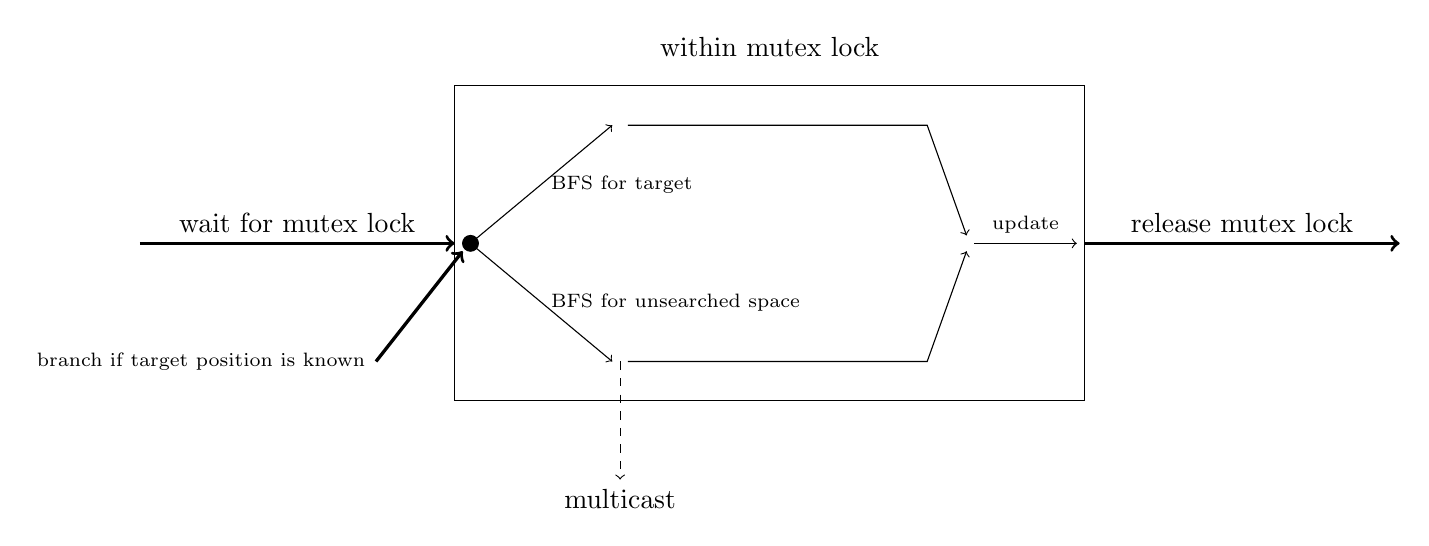
\begin{tikzpicture}
    \draw[->,very thick] (-4,2) -- (0,2) node[pos=0.5,above]
      {wait for mutex lock};
    \draw (0,0) rectangle (8,4) node[pos=0.5,yshift=2.5cm] {within mutex lock};
    \draw[->,very thick] (8,2) -- (12,2) node[pos=0.5,above]
      {release mutex lock};
    \draw[fill] (0.2,2) circle (0.1cm);
    \draw[<-,very thick] (0.1,1.9) -- (-1,0.5) node[left]
      {\scriptsize{branch if target position is known}};
    \draw[->] (0.2,2) -- (2,0.5) node[pos=0.5,right]
      {\scriptsize{BFS for unsearched space}};
    \draw[dashed,->] (2.1,0.5) -- (2.1,-1) node[below] {multicast};
    \draw[->] (0.2,2) -- (2,3.5) node[pos=0.5,right]
      {\scriptsize{BFS for target}};
    \draw[->] (2.2,0.5) -- (6,0.5) -- (6.5,1.9);
    \draw[->] (2.2,3.5) -- (6,3.5) -- (6.5,2.1);
    \draw[->] (6.6,2) -- (7.9,2) node[pos=0.5,above] {\scriptsize{update}};
  \end{tikzpicture}
\end{center}

\subsubsection*{A Single Update Cycle}
\begin{center}
  \begin{tikzpicture}
    \draw[->] (0,4) -- (3,4) node[pos=0.5,above]
      {\scriptsize{update cycle begins}};
    \foreach \y in {0,2,6,8} {
      \draw[->] (3.1,4) -- (5,\y);
      \draw (5.1,\y-0.5) rectangle (8,\y+0.5);
      \draw (8.1,\y) -- (10,4);
    }
    \node[left] at (4.5,7) {\scriptsize{wait for mutex lock}};
    \node[right] at (5.2,0) {Robot \( k \)};
    \node[right] at (5.2,2) {Robot \( k-1 \)};
    \node[right] at (5.2,4) {\large{\( \vdots \)}};
    \node[right] at (5.2,6) {Robot 2};
    \node[right] at (5.2,8) {Robot 1};
    \draw[dashed,->,very thick] (5.5,7.5) .. controls (6,4) .. (5.5,0.5);
    \draw[dashed,->,very thick] (5.5,7.5) .. controls (6.5,5) .. (6.5,2.5)
      node[pos=0.6,right] {multicast};
    \draw[dashed,->,very thick] (5.5,7.5) -- (6.5,6.5);
    \draw (10,3.5) rectangle (12.5,4.5) node[yshift=-0.5cm,left] {\scriptsize{draw to output}};
    \draw[->] (12.5,4) -- (15.5,4) node[pos=0.5,above]
      {\scriptsize{update cycle ends}};
  \end{tikzpicture}
\end{center}
During the update cycle, each robot maintains whether or not it has updated
during that cycle. If it has already updated, then it will not update again
until the next update cycle begins. This ensures that each robot updates once
during each cycle and has a chance to move one square. The only exception to
this occurs if the robots are in the convergence phase, since robots that are
``done'' will be skipped by this update counter. \par
Since the state of the grid is stable at the end of each update cycle, we draw
the state of the grid at the end of each update cycle. The robots use an
election process to delegate drawing to the \textit{last} robot that updates
during each update cycle.

\subsection*{Results}
To run the simulation, compile the program by invoking \texttt{make} in the
program directory, and then invoke the \texttt{simulate} executable. The
executable takes 3 parameters and an optional random seed. Note that the delay
represents a minimum delay in milliseconds between each update cycle. \\ \\
\texttt{./simulate <grid size> <robots> <delay> [seed]} \\ \\
In the simulation, each robot is denoted by a letter that uniquely identifies
it. The grid itself is bounded with the \texttt{=} and \texttt{|} characters,
while the target block is identified with that \texttt{\#} character. Squares
that the robots have searched are marked with the \texttt{-} character. \par
Given a grid size \( l\times b \) with \( k \) robots, the search phase's
running time is upper bounded by \( \frac{lb}{k} \) steps. Once a robot finds
the target block, it communicates the position via multicast and all robots
begin the convergence phase. The convergence phase's running time is bounded by
\( l+b \) since that is the maximum possible distance a robot may need to travel
to reach the target block. In terms of steps taken, the simulation runs in
\( O(\frac{lb}{k}+l+b) \) time.

\end{document}
